\label{chapter:nq}

\section{The Story of Natural Questions}

My goal with this video is to give an overview of the kinds of question answering datasets that are out there, contrast them, and give my opinion about which is the best one.

First, let me start off by saying what we're not talking about!  There are many question answering datasets out there that are essentially logic problems or SQL query lookups and we're not going to talk about them.  That's a very valid form of question answering and it essentially corresponds to a form of parsing where you have some text and you need to turn that into a logical form or an SQL statement.  If you parse it correctly, you get the answer.

Instead, we're going to talk about more open-ended question answering that’s often called “machine reading” question answering for reasons that will be clear in a second.  In these question answering datasets, you need to make sense of a large body of text to answer questions.  Moreover, you usually need to be able to answer questions about just about anything, not just a narrow set of topics.

We'll talk about models for answering these questions later, but for the moment think about the kinds of things that your model would need to do to answer the question.  In many cases, it will be exactly the same kind of thing you would need to do to answer the question: find a document that contains the answer, read through the document to find the answer, and then convey that answer.

Okay, back to the datasets.  Rather than just listing them off, I’m going to try to organize the datasets based on: how much information you have to answer the question and how complicated the answer is.  Let’s say that we can write this as a two dimensional plot with provided information as the x axis and answer complexity as the y axis.  I’ll roughly go chronologically through time.

In another video, there’s another important dimension: who’s writing the question and for what purpose, but I think that’s so important that I want to focus on it by itself.  So if you’re interested in that, check out the Cranfield vs. Manchester discussion linked in the description. 

Let’s start with the most simple example of a question answering dataset: you get a question as input and you need to produce a short answer.  This is often called factoid QA.  The prototypical example of this is TREC QA.  This is a super old school dataset, but important to remember, as it set the form of everything that came after.

The actual dataset is tiny: only a couple hundred questions.  And the official evaluation process seems impossible by today’s standards: you had professional annotators judge whether a system provided the right answer.  While every other dataset we’ll talk about has more automatic evaluations, this is probably the best way to do it, at least for some trickier answers.

This is our first QA dataset, so let’s put this onto the board here.  Let’s now go into the modern age!

One of the first machine reading data sets was the CNN / Daily Mail data set from Karl Moritz Hermann and company.  Here you have a bunch of news articles.  This dataset started the trend of conditioning a question on a document: in this case a news article.  They asked you to answer questions about those news articles.  For example, “who reached the Cricket World Cup”.  Somewhere in the document was the answer “New Zealand” but you need to find that.

One thing that is controversial is that you didn’t actually find the string “New Zealand” but rather an anonymized symbol.  This meant that you couldn’t just have a language model memorize all the answers (which is even more of a problem now that it was back then).  However, this had another drawback!  Because there weren’t that many symbols, the task was essentially a multiple-choice question: you identified the entities in the paragraph and then you picked which one was correct.  Despite this problem and and that introduced a little bit of noise to the problem, you can see the influence of this question answering dataset on the rest of the field, particularly on “the next big thing”: SQuAD.

The Stanford question answering dataset has become the gold standard.  While it might not be the best dataset, it’s the most popular.  If you don't report results on SQuAD, you need to explain why.  This 2016 dataset set helped popularized the modern upsurge of question answering.  These questions use paragraphs from Wikipedia ask crowd workers to write questions about that paragraph.  The questions are intended to have an answer that is a span within that Wikipedia paragraph.  One way of thinking about this is that a span is a contiguous span of characters: you highlight that span to give the answer.

This is a very large data set so it doesn't have many of the problems of the smaller data sets that we've talked about before. The downside of this is that these crowd workers can often be reverse engineered there are tricks and cheats that they use to create questions.  For example, if a question asks “when”, then all a QA system really has to do is find the thing that is being asked about and then find the closest thing that looks like a date nearby.  In other words, the machine learning algorithms are essentially reverse engineering those annotators rather than solving the intrinsic problem.

The real reason, in my opinion, that squad has become the gold standard is that it has a very well trafficked leaderboard where people can submit their systems and to see how they stack up against the rest of the world.  Because the answers are spans within the original document this reduces the task to multiple-choice much like the Daily Mail/CNN data set that we talked before.  Thus, it doesn't allow answers that are latent in the text that aren’t a fixed span.  For example, if the question is “What states share the Delmarva peninsula with Maryland” and the Wikipedia page has “The Delmarva peninsula is made up of Deleware, Maryland, and Virginia”, it can’t answer “Delaware and Virigina” because there’s a pesky Maryland in the middle!

One thing that really grinds my gears about SQuAD is that the SQuAD dataset provides a “human upper bound” (and to be clear this is not the fault of the people who designed SQuAD but from people who misinterpret what they did) but there less well informed news organizations or promoters of research that mischaracterize what it means to be near the human bound.  It also mischaracterizes what it means to “read” a document.  If machine learning systems are getting close to this human bound it doesn't mean that computers are reading better than humans.  Rather, it means that computers are doing a better job of highlighting particular passages better than underpaid crowd workers.  I’ll talk more about what I think is a fair human comparison in a moment.

So putting this on the chart, I’m going to put SQuAD a little bit above CNN/DailyMail.  They’re both implicitly multiple choice, but there are more spans than entities, so answering SQuAD questions is a little more difficult.

One criticism of SQuAD questions is that their questions are unnatural.  They’re written by crowdworkers paid to write artificial questions.  Two datasets that use “real” questions are MS Marco and Natural Questions.  They’re both somewhat similar, so I’ll mostly talk about Natural Questions, which is newer as a stand-in for both.  These questions are harder than SQuAD and Trec questions!  That’s because the questions come from people using search engines.  These people don’t always know what they’re asking about (that’s why their using a search engine after all), so sometimes they have false assumptions, ambiguities, and other problems.  

Another facet of these datasets that make the questions harder is that search engines have trained people over years to answer questions themselves by finding webpages.  Nobody gets good answers when they type in a question like “what is the last capital in Western Europe to be invaded by a foreign army” so if you type that into Google you likely will not get an answer to that question directly.  Instead, you’ll piece together multiple queries to answer your question.

In other words, the failure of search engines to answer questions over the last couple of decades limits the usefulness of the kinds of questions that you can get from search engines today.  

So how does Natural Questions find the answers to these questions?  They find Wikipedia given the question as a search string: an information retrieval problem!  They then have annotators validate that this is a good search result and then have the annotators highlight the answer string.  Now this isn’t perfect.  

Here are some examples where I disagree with some of the implicit assumptions that get made in the NQ dataset.  For example, it assumes that when you’re asking about “Michigan”, you’re asking about the “university of michigan football team”, when you’re asking about “hockey”, you’re asking about “men’s ice hockey”, and when you’re asking about “supreme court” you’re asking about the “indian supreme court”.  

As we put these datasets up on the chart, I want to make a distinction between the “Traditional” and “Open” interpretations of natural questions.  While initial natural questions was treated as a SQuAD-like dataset, recent interpretations have not assumed that you know which Wikipedia page had the answer: you also need to do the IR component as well.  This is what we did in the EfficientQA competition (link in the description): you can see how I made the human vs. computer comparison a little more fair.

Obviously, the open interpretation makes it much harder to find the answer.


Moving on … You know who’s better than underpaid crowd workers or random people on the Internet?  Professional trivia writers.  And a number of datasets use questions harvested from them.

Let’s talk about three of them: SearchQA, TriviaQA, and Quiz Bowl.

SearchQA and TriviaQA actually look a lot like Natural Questions, but instead of the queries coming from random people on the internet, they come from professional writers.  Researchers go out and find pages given the query, highlight the answers.  I’m not going to dwell too much on these datasets because the copyright is a little murky.

Instead, let's now turn to my hobby horse: quiz bowl, which is probably best known as an NBC game show in the US called “college bowl” and “University Challenge” in the UK.  And played by thousands of trivia nerds every weekend, particularly at the high school and college level.  And unlike SearchQA and TriviaQA, there’s an explicit community consensus that old quiz bowl questions are public domain.  So as a result we get a lot of free data from experts. These are not crowd workers: these are people who are passionate about human question answering, and we're using their expertise and their experience to improve computer question answering.

This is the gold standard in human question answering (i.e., trivia tournaments), and my goal is to make it more popular than it currently is for computer question answering.  What’s different about quiz bowl is that there isn’t just one question that you need to answer.  Instead, there are multiple clues that you could use to answer the question.  

This is hard to explain, so let’s see an example.  As I read it, think about when you know the answer to the question.  What clue gave it away?

While passing through this state, the 6th Massachusetts
suffered the first Union casualties of the Civil War while
suppressing riots that began at its President Street
Station. The Lincoln administration rejected a ruling by
Roger Taney that a citizen of this state could not
be held without habeas corpus in the case Ex Parte
Merryman. After capturing a copy of Robert E. Lee’s
Special Order 191, George McClellan fought a battle in
this state that ended the first Confederate invasion of
the North and led to the announcement of the
Emancipation Proclamation. For 10 points, the Battle of
Antietam was fought in what border state where federal
troops blocked secessionist efforts in Baltimore?



The clues are presented one by one until someone can answer the question with the great state of Maryland. Because this is a competition, whoever can answer the question faster (on harder clues) usually knows more about the topic.  Because this is a trivia game, the goal is to give more points to the smarter player.  Quiz bowl does this really well!  Better than some other fun to watch knowledge competitions.

The downside is that sometimes what's difficult for a human isn't difficult for a computer and—just like squad—there sometimes easily solved questions that are intended to be difficult (for humans) but aren't actually difficult (for computers).  

For example, in one of the early competitions we had with humans, a computer could easily recognize a painting from a description. 

But computers struggle with simple language, 

The computer incorrectly thinks that when the question says “this author opens Crime and Punishment” that the answer is Dostoyevski.

As you can tell from these clips, one of the reasons that I’m a big fan of this competition is that it lends itself to comparisons. Let’s say you have two competitors A and B. What if we try to compare them on normal questions like from natural questions? If both get the question right or wrong, you don’t learn anything. You only learn something if one gets it right and the other gets it wrong. Human question writers learned really early on that it’s really hard to get the level of difficulty just right: even with fancy statistics, you need hundreds of questions to reliably rank people in competitive exams.

So this is why the human trivia community turned to quiz bowl. Instead of just getting one piece of information per question, you now potentially get a signal from every word in the question. Because the questions are packed to the gills with clues that go from super difficult to to almost painfully easy, after each clue you get information about how much A and B knows. Thus, it lends itself to human-computer competition or comparing computer systems.

Another reason that I like quiz bowl is that there are multiple ways to approach it computationally. Because the answers are usually entities, you can take a straight information retrieval approach: what’s being talked about in this question? Or you can take a more machine reading approach. Both work well!

Okay, that’s enough about quiz bowl. Let’s put it on the board: the answer structure is about the same as NQ, but the question structure is very complicated.

\jbgcomment{Work on this chapter in conjunction with iid draft}

\section{Natural Questions Five Years Later}
\label{sec:nq:problems}

It’s been five years since Natural Questions came out.  It’s hard to overstate its impact on Question Answering (QA).  Perhaps only second to SQuAD.  SQuAD introduced the extractive format, but SQuAD was “fake” … Natural Questions had true complexity and verisimilitude: people ask crazy questions, some of the questions were unanswerable, and the answers were tied to Wikipedia pages.  And it has yet to be eclipsed … and perhaps it never will.  

Part of the reason that this will probably never happen again is that Natural Questions has two very unique characteristics: questions from real users expensively verified by expensive annotators.  While it’s possible that we might get something like this again in part—UW folks crawled Google n-grams to extract the questions, we paid QuizBowlers to find passages to answer questions—getting them both at once is probably not going to happen again.  But I’d love to be proved wrong!  I’ll end the video with how I’d build a QA dataset with infinite resources.

However, Natural Questions aren’t perfect.  Sewon Min and company created AmbigQA that showed some of the questions in Natural Questions were ambiguous.  Here are some examples that Ben and I talked about in our 2020 paper (and I talked about at more length in the QA datasets lecture, link in the description).  There are multiple interpretations to these questions, but Natural Questions only says that one of them is correct.  

How is the “correct” interpretation chosen in the original Natural Questions paper?  The annotators saw search results from an information retrieval system, and if they found an answer there, they called it the correct answer.  So whatever process biases search results toward English-speaking judges, men’s sports, or flagship universities gets recapitulated in Natural Questions.

Another development is the realization that not all questions are valid and shouldn’t be answered.  There are multiple aspects of this: appropriately calibrating your QA system to abstain when it doesn’t know the answer for example.  Natural Questions actually does a pretty good job of supporting this by having unanswerable questions.

But instead, I want to focus on linguistic phenomena that *causes* a question to *become* unanswerable.  This line of research began with what has come to be known as as “the lightbulb paper” from the title “Which linguist invented the lightbulb”, which highlights the problem: there’s a well-defined answer to the question “who invented the first commercially successful light bulb”, but it sure as heck wasn’t a linguist … answering that question would perhaps not be useful to a user.

There are two takeaways here: First that many QA systems tend to roll with questions like “When did Pablo Picasso paint the Mona Lisa” and answer 1503, hundreds of years before Picasso was born.  Second, that many of the unanswerable questions in Natural Questions are unanswerable because of these phenomena.  And it’s not just Natural Questions: Yu et al showed that this also shows up on Reddit.  It’s an important problem!

But we don’t actually know *why* a particular natural question is unanswerable.  Is it because Wikipedia lacks the information, because there’s a false assumption, because there’s actually dispute about the canonical answer to a question, or because it’s a matter of taste / opinion?  Because Natural Questions was focused on factual QA (a reasonable position five years ago), we don’t have a single comprehensive dataset to address all of these issues (the numbers here are just for a small sample of NQ).

And perhaps we don’t need that any more.  With RLHF, we can just mix a bunch of datasets together.  Perhaps we don’t need a monolithic QA training dataset to rule them all.  We just need robust evaluation protocols (which can be much smaller). 

And this is, again, a weakness of Natural Questions … it’s not a great evaluation set.  Lewis et al. discovered that many QA datasets, including Natural Questions, have a huge overlap between the training set and the testing set.  I’m a Professor, so let’s put this in a classroom context: this is like giving out two thirds of the answers and one third of the questions as a study guide before the test.  Now, it’s a great sanity check that systems can answer those questions, but that means that only a third of the questions are part of a functional test set.  Add that to the problems of ambiguity, and far less of the test set is actually usable, making it difficult to know if we’re making progress on the dataset.

This is something that the trivia community has known for a while.  You can’t reuse clues!  For important test sets (like national trivia tournaments), you need to make sure that you’re finding new, interesting clues that haven’t been used before (or at least for a while).  This is why we’ve always used the flagship national trivia tournaments as our test sets for quiz bowl.

So that’s all I have about the problems of Natural Questions.  But I want to make it clear that *Natural Questions remains a great resource*.  It hasn’t been matched.  I still use it.  I’m jealous of the people who got to build it.  But it’s important to know the limitations.  Is there anything I got wrong, anything I missed?  If so, let me know in the comments.

Now, for all of the reasons I talked about before, it probably will never be done again.  Nobody is crazy enough to do it.  But how would I do it if someone were foolish enough to give me the resources to create the next iteration of something like it?

Back in the early 2000s, there was a QA service called Aardvark.  The idea was that it would connect up real humans with topics those smart humans could answer questions about.  Question comes in and it gets routed to that person.  That was a great idea but before it’s time.  What you’d do today is build up a large collection of these people (and pay them well), a question from a major search engine comes in … we try to detect if the computer can answer it directly.  If yes, we answer it, if not, we farm it out to the experts.  We’ve trained the experts to interrogate the question askers to remove ambiguities, false presuppositions, etc.  To create a “clean” version of the question and then a strong reference answer supported by relevant information.

Yogesh Raut’s recreational thinking podcast is an example of this interrogation process: they spend several minutes interrogating individual questions, figuring out possibilities, and then justifying the answer.

So for example, if the question comes in: “What linguist invented the lightbulb”, you might have an interaction that goes like this:

“Um, actually, most of the people credited with the development of the lightbulb were chemists, physicists, or engineers”

“Okay, smartbutt, who made the first lightbulb”

“Well, do you mean created the first electric light (Humphry Davy), the first filament inside a vacuum tube (Jospeh Swan), the first metal filament in a vacuum tube (Warren de la Rue), or the first commercially successful lightbulb with those properties (Thomas Edison)?”

“Hmm … I guess I meant who got the credit for it”

“Then that would be Thomas Edison”

And to be clear, that’s not what happens if you ask this to ChatGPT … it doesn’t really probe the user’s intent but tries to do some correction (not invented by a linguist) and provide the answer to the most likely question.  But still erases all of the people whose work Edison built on.

But we can build such a system—again, my DMs are open—Natural Questions are still the best we have.

\section{Is \abr{iid} the Right Choice of Data?}
\label{sec:nq:iid}

Creating new machine learning systems requires data.  These data need to come
from somewhere, and NLP systems are no different!  If you were to ask a
statistician, they would tell you get a sample from an \iid{} distribution:
independent and identically distributed.  Independent means that example
$x_{n}$ does not depend on on any of the previous examples 1 to n-1, indeed,
all of the examples come from the *same* underlying distribution.

But that’s the problem.  Language isn’t like neutrinos spewed from the sun or
water from a geyser.  Language is inherently an interactive process: and what
I’m going to argue is that this has always been a problem for our NLP
datasets, that it’s getting worse with the advent of muppet Models, and that
we need to address the problem head on going forward.

\subsection{The Ghost of NLP Data Past}

One of the biggest sources of NLP data are crowdworkers.  These are not iid!  Crowdworkers are not representative of the global population: by definition they have access to a computer, they’re typically younger, and they’re focused in particular geographic areas.

And even if you restrict to US Crowdworkers (because nobody has virtual private networks or virtual credit cards), this distribution does not match the overall US population.

And beyond the underlying distribution issue, there’s a quality issue.  Crowdsourced data often has “shortcuts” that allow systems to “cheat”.  We’ve seen this for:
Entailment: systems can detect whether a claim is true or not just by looking at the premise or the hypothesis (when you should really need both).  Grurangan et al show that crowdworkers use the same tricks to create examples: “at least” is often entailed, irrelevant information is often neutral, and negation is often contradicted.  Poliak et al showed that you can get pretty high accuracy by ignoring the premise and characterized the “tells” that often appeared in the data. And we had our own paper that even when the premise is required, it doesn’t require deep reasoning.
For fact checking: like with entailment, some logical operators like negations are more likely associated with refutation.  We talked about this in our adversarial fact checking paper, Fool Me Twice.
and for question answering: for datasets like SQuAD, the answer selection process often didn’t need deep understanding of the source context as described by Weissenborn et al.  Look at the passage and find the first thing that could possibly fit the answer type: When finds the year, who finds a person, where finds a place, etc.  

This is because crowdworkers had to look at a passage and generate a question that could be answered by that passage.  The questions didn’t require that much reasoning because the Crowdworkers wanted to get done as quickly as possible.

Speaking of question answering, natural questions claim to be “natural” … these are the data from real users, this actually is iid right?  And I think the answer is no!  This is because all language is a negotiation—a give and take between two parties—and Google is a part of that negotiation. 

Now, Google is a fantastic tool, but it has its strengths and weaknesses.  It’s really good at looking up who played role X in movie Y.  IMDB (and other structured knowledge bases) make answering this kind of question easy … so people know that if they ask this kind of question from Google they’re likely to get a good answer.  In general, if I can clearly specify entity X and a relationship f(X) that’s going to appear in some KB, then I’m going to get a great answer.

So this means that people are more likely to ask this kind of question.  But longer questions just harder to answer.  People want to get answers to their questions, so Google has trained users over the last 25 years to ask the kinds of things it can answer (and the average length of queries is going up!).  But at the end of the day, the kinds of questions that Google isn’t so good at are not going to be asked so they’re not going to be a part of the dataset.  And that means that it won’t be part of the all important natural questions leaderboard.  Which means that people will ignore the questions that Google isn’t already good at.

Now, Jordan, aren’t you just being a meanie by picking on Natural Questions?  Your favorite QA dataset that you keep pushing down everybody’s throat—quiz bowl—ain’t iid either.  

And that’s absolutely right!  I like these crazy quiz bowl questions where the distribution has been chosen by hand to reflect the undergraduate curriculum at American Universities.  This also isn’t iid, but I think specifying the distribution and being able to defend it is a good thing!

And in addition to the “kinds” of questions in Natural Questions, Google has trained users to ask questions in a particular way: instead of asking “who is Amal Alamuddin’s husband”, people type “Amal Alamuddin husband” because Google started as a search engine that ignored function words.  So this also affects what gets into natural questions: Google has trained people to write terse queries, NQ subselects from that, and that becomes the leaderboard.

From a socio-technical perspective, Google is to the turn of the century like muppet models are to today [link in the description if you don’t know why I call things like GPT Muppet Models].  People are learning how to skillfully prompt muppet models, muppet models are impersonating humans on crowdworking platforms (another reason that datasets from crowdworkers aren’t iid), people are using them to help write their essays (which will in turn be used to train the next generation of muppet models when those essays get posted on the web).  

So what does this mean?  

Okay, so I’m going to get on my soapbox for a bit … we need to embrace the interaction between users and systems.  And that means something like adversarial examples which we’ll talk about later in later lectures … link to a lecture if you’re impatient.  But the basic idea is that you have humans and models interact with each other to create examples that “push the frontier” of what’s possible.

Sam Bowman in his paper about the dangers of underclaiming … if you do research on adversarial data, the accuracy numbers are going to be lower than “normal” datasets.  But I think that this makes a category error!  There’s no such thing as a normal, iid dataset.  All datasets have their own pathologies, and you cannot readily compare SQuAD numbers to NQ numbers: there are fundamentally different underlying distributions and data collection practices.  The same thing is true for my beloved quiz bowl format.

And I think this is a healthy development.  Rather than obsessing about rank on a leaderboard and the single floating point number with your accuracy that comes out, we should focus on what are the abilities (and weaknesses) of models.  And accepting that there is no such thing as the iid language bunny bringing you a basket of nicely distributed questions will help us get there faster.

My goal with this video is to give an overview of the kinds of question answering datasets that are out there, contrast them, and give my opinion about which is the best one.

First, let me start off by saying what we're not talking about!  There are many question answering datasets out there that are essentially logic problems or SQL query lookups and we're not going to talk about them.  That's a very valid form of question answering and it essentially corresponds to a form of parsing where you have some text and you need to turn that into a logical form or an SQL statement.  If you parse it correctly, you get the answer.

Instead, we're going to talk about more open-ended question answering that’s often called “machine reading” question answering for reasons that will be clear in a second.  In these question answering datasets, you need to make sense of a large body of text to answer questions.  Moreover, you usually need to be able to answer questions about just about anything, not just a narrow set of topics.

We'll talk about models for answering these questions later, but for the moment think about the kinds of things that your model would need to do to answer the question.  In many cases, it will be exactly the same kind of thing you would need to do to answer the question: find a document that contains the answer, read through the document to find the answer, and then convey that answer.

Okay, back to the datasets.  Rather than just listing them off, I’m going to try to organize the datasets based on: how much information you have to answer the question and how complicated the answer is.  Let’s say that we can write this as a two dimensional plot with provided information as the x axis and answer complexity as the y axis.  I’ll roughly go chronologically through time.

In another video, there’s another important dimension: who’s writing the question and for what purpose, but I think that’s so important that I want to focus on it by itself.  So if you’re interested in that, check out the Cranfield vs. Manchester discussion linked in the description. 

Let’s start with the most simple example of a question answering dataset: you get a question as input and you need to produce a short answer.  This is often called factoid QA.  The prototypical example of this is TREC QA.  This is a super old school dataset, but important to remember, as it set the form of everything that came after.

The actual dataset is tiny: only a couple hundred questions.  And the official evaluation process seems impossible by today’s standards: you had professional annotators judge whether a system provided the right answer.  While every other dataset we’ll talk about has more automatic evaluations, this is probably the best way to do it, at least for some trickier answers.

This is our first QA dataset, so let’s put this onto the board here.  Let’s now go into the modern age!

One of the first machine reading data sets was the CNN / Daily Mail data set from Karl Moritz Hermann and company.  Here you have a bunch of news articles.  This dataset started the trend of conditioning a question on a document: in this case a news article.  They asked you to answer questions about those news articles.  For example, “who reached the Cricket World Cup”.  Somewhere in the document was the answer “New Zealand” but you need to find that.

One thing that is controversial is that you didn’t actually find the string “New Zealand” but rather an anonymized symbol.  This meant that you couldn’t just have a language model memorize all the answers (which is even more of a problem now that it was back then).  However, this had another drawback!  Because there weren’t that many symbols, the task was essentially a multiple-choice question: you identified the entities in the paragraph and then you picked which one was correct.  Despite this problem and and that introduced a little bit of noise to the problem, you can see the influence of this question answering dataset on the rest of the field, particularly on “the next big thing”: SQuAD.

The Stanford question answering dataset has become the gold standard.  While it might not be the best dataset, it’s the most popular.  If you don't report results on SQuAD, you need to explain why.  This 2016 dataset set helped popularized the modern upsurge of question answering.  These questions use paragraphs from Wikipedia ask crowd workers to write questions about that paragraph.  The questions are intended to have an answer that is a span within that Wikipedia paragraph.  One way of thinking about this is that a span is a contiguous span of characters: you highlight that span to give the answer.

This is a very large data set so it doesn't have many of the problems of the smaller data sets that we've talked about before. The downside of this is that these crowd workers can often be reverse engineered there are tricks and cheats that they use to create questions.  For example, if a question asks “when”, then all a QA system really has to do is find the thing that is being asked about and then find the closest thing that looks like a date nearby.  In other words, the machine learning algorithms are essentially reverse engineering those annotators rather than solving the intrinsic problem.

The real reason, in my opinion, that squad has become the gold standard is that it has a very well trafficked leaderboard where people can submit their systems and to see how they stack up against the rest of the world.  Because the answers are spans within the original document this reduces the task to multiple-choice much like the Daily Mail/CNN data set that we talked before.  Thus, it doesn't allow answers that are latent in the text that aren’t a fixed span.  For example, if the question is “What states share the Delmarva peninsula with Maryland” and the Wikipedia page has “The Delmarva peninsula is made up of Deleware, Maryland, and Virginia”, it can’t answer “Delaware and Virigina” because there’s a pesky Maryland in the middle!

One thing that really grinds my gears about SQuAD is that the SQuAD dataset provides a “human upper bound” (and to be clear this is not the fault of the people who designed SQuAD but from people who misinterpret what they did) but there less well informed news organizations or promoters of research that mischaracterize what it means to be near the human bound.  It also mischaracterizes what it means to “read” a document.  If machine learning systems are getting close to this human bound it doesn't mean that computers are reading better than humans.  Rather, it means that computers are doing a better job of highlighting particular passages better than underpaid crowd workers.  I’ll talk more about what I think is a fair human comparison in a moment.

So putting this on the chart, I’m going to put SQuAD a little bit above CNN/DailyMail.  They’re both implicitly multiple choice, but there are more spans than entities, so answering SQuAD questions is a little more difficult.

One criticism of SQuAD questions is that their questions are unnatural.  They’re written by crowdworkers paid to write artificial questions.  Two datasets that use “real” questions are MS Marco and Natural Questions.  They’re both somewhat similar, so I’ll mostly talk about Natural Questions, which is newer as a stand-in for both.  These questions are harder than SQuAD and Trec questions!  That’s because the questions come from people using search engines.  These people don’t always know what they’re asking about (that’s why their using a search engine after all), so sometimes they have false assumptions, ambiguities, and other problems.  

Another facet of these datasets that make the questions harder is that search engines have trained people over years to answer questions themselves by finding webpages.  Nobody gets good answers when they type in a question like “what is the last capital in Western Europe to be invaded by a foreign army” so if you type that into Google you likely will not get an answer to that question directly.  Instead, you’ll piece together multiple queries to answer your question.

In other words, the failure of search engines to answer questions over the last couple of decades limits the usefulness of the kinds of questions that you can get from search engines today.  

So how does Natural Questions find the answers to these questions?  They find Wikipedia given the question as a search string: an information retrieval problem!  They then have annotators validate that this is a good search result and then have the annotators highlight the answer string.  Now this isn’t perfect.  

Here are some examples where I disagree with some of the implicit assumptions that get made in the NQ dataset.  For example, it assumes that when you’re asking about “Michigan”, you’re asking about the “university of michigan football team”, when you’re asking about “hockey”, you’re asking about “men’s ice hockey”, and when you’re asking about “supreme court” you’re asking about the “indian supreme court”.  

As we put these datasets up on the chart, I want to make a distinction between the “Traditional” and “Open” interpretations of natural questions.  While initial natural questions was treated as a SQuAD-like dataset, recent interpretations have not assumed that you know which Wikipedia page had the answer: you also need to do the IR component as well.  This is what we did in the EfficientQA competition (link in the description): you can see how I made the human vs. computer comparison a little more fair.

Obviously, the open interpretation makes it much harder to find the answer.


Moving on … You know who’s better than underpaid crowd workers or random people on the Internet?  Professional trivia writers.  And a number of datasets use questions harvested from them.

Let’s talk about three of them: SearchQA, TriviaQA, and Quiz Bowl.

SearchQA and TriviaQA actually look a lot like Natural Questions, but instead of the queries coming from random people on the internet, they come from professional writers.  Researchers go out and find pages given the query, highlight the answers.  I’m not going to dwell too much on these datasets because the copyright is a little murky.

Instead, let's now turn to my hobby horse: quiz bowl, which is probably best known as an NBC game show in the US called “college bowl” and “University Challenge” in the UK.  And played by thousands of trivia nerds every weekend, particularly at the high school and college level.  And unlike SearchQA and TriviaQA, there’s an explicit community consensus that old quiz bowl questions are public domain.  So as a result we get a lot of free data from experts. These are not crowd workers: these are people who are passionate about human question answering, and we're using their expertise and their experience to improve computer question answering.

This is the gold standard in human question answering (i.e., trivia tournaments), and my goal is to make it more popular than it currently is for computer question answering.  What’s different about quiz bowl is that there isn’t just one question that you need to answer.  Instead, there are multiple clues that you could use to answer the question.  

This is hard to explain, so let’s see an example.  As I read it, think about when you know the answer to the question.  What clue gave it away?

While passing through this state, the 6th Massachusetts
suffered the first Union casualties of the Civil War while
suppressing riots that began at its President Street
Station. The Lincoln administration rejected a ruling by
Roger Taney that a citizen of this state could not
be held without habeas corpus in the case Ex Parte
Merryman. After capturing a copy of Robert E. Lee’s
Special Order 191, George McClellan fought a battle in
this state that ended the first Confederate invasion of
the North and led to the announcement of the
Emancipation Proclamation. For 10 points, the Battle of
Antietam was fought in what border state where federal
troops blocked secessionist efforts in Baltimore?



The clues are presented one by one until someone can answer the question with the great state of Maryland. Because this is a competition, whoever can answer the question faster (on harder clues) usually knows more about the topic.  Because this is a trivia game, the goal is to give more points to the smarter player.  Quiz bowl does this really well!  Better than some other fun to watch knowledge competitions.

The downside is that sometimes what's difficult for a human isn't difficult for a computer and—just like squad—there sometimes easily solved questions that are intended to be difficult (for humans) but aren't actually difficult (for computers).  

For example, in one of the early competitions we had with humans, a computer could easily recognize a painting from a description. 

But computers struggle with simple language, 

The computer incorrectly thinks that when the question says “this author opens Crime and Punishment” that the answer is Dostoyevski.

As you can tell from these clips, one of the reasons that I’m a big fan of this competition is that it lends itself to comparisons. Let’s say you have two competitors A and B. What if we try to compare them on normal questions like from natural questions? If both get the question right or wrong, you don’t learn anything. You only learn something if one gets it right and the other gets it wrong. Human question writers learned really early on that it’s really hard to get the level of difficulty just right: even with fancy statistics, you need hundreds of questions to reliably rank people in competitive exams.

So this is why the human trivia community turned to quiz bowl. Instead of just getting one piece of information per question, you now potentially get a signal from every word in the question. Because the questions are packed to the gills with clues that go from super difficult to to almost painfully easy, after each clue you get information about how much A and B knows. Thus, it lends itself to human-computer competition or comparing computer systems.

Another reason that I like quiz bowl is that there are multiple ways to approach it computationally. Because the answers are usually entities, you can take a straight information retrieval approach: what’s being talked about in this question? Or you can take a more machine reading approach. Both work well!

Okay, that’s enough about quiz bowl. Let’s put it on the board: the answer structure is about the same as NQ, but the question structure is very complicated.

If you subscribe to this channel, you’ll hear about it often enough (and see matches between humans and computers). 

Before we wrap up, I want to talk about a bunch of other datasets really quickly.  I won’t discuss them in detail and I won’t talk about all of the QA datasets out there … there are just too many these days!  But if any of these sound interesting to you or if I’ve left out a favorite, put a link in the comments!

QuAC: This dataset is about conversational question answering. As a result, many of the questions depend on coreference or other ambiguities. We created a version called CANARD to remove those ambiguities. And our QBLink does something similar with quiz bowl questions.

NarrativeQA: This is a great dataset, but it’s not as popular as it should be because it’s just too darn hard. You have a script of an interaction and you need to answer a question about what happened in the story. It doesn’t lend itself to the machine reading approaches that work for other datasets.

HotPotQA: Requires you to string together multiple pieces of information to answer the question. This is implicitly in a lot of quiz bowl questions but not annotated except in a small subset of questions in a Guha et al 2015 dataset. The authors of HotPotQA got authors to explicitly mark what the answer is to the internal questions.

Also, there are whole types of question answering that I haven’t talked about at all. What about non-English datasets? There are a few (but not enough). What about answering questions about pictures? There are datasets for those, but this video is already long enough as it is. 

So I should probably wrap up for real. Question answering is a really exciting field right now. There’s so much energy both from people building datasets and models. And despite my enthusiasm for quiz bowl, I also recognize that it’s not the perfect format.  But because ML datasets need training data to improve, before we create machines that can answer any question, we first need to create datasets that will teach the machines.

\section{Surprise, this is a Trivia Tournament!}
\label{sec:tournament}


``My research isn't a silly trivia tournament,'' you say.
That may be, but let us first tell you a little about what running a tournament is like, and perhaps you might see similarities.


First, the questions.
Either you write them yourself or you pay someone to write questions by a particular date (sometimes people on the Internet). 

Then, you advertise.  
You talk about your questions:
who is writing them, what subjects are covered, and why people should try to answer them.

Next, you have the tournament. 
You keep your questions secure until test time, collect answers from all participants, and declare a winner. 
Afterward, people use the questions to train for future tournaments.

These have natural analogs to crowd sourcing questions, writing the paper, advertising, and running a leaderboard. 
Trivia nerds cannot help you form hypotheses or write your paper, but they can tell you how to run a fun, well-calibrated, and discriminative tournament.

Such tournaments are designed to effectively find a winner, which matches the scientific goal of knowing which model best answers questions.
Our goal is {\bf not to encourage the \abr{qa} community to adopt the quirks and gimmicks of trivia games}.
Instead, it's to encourage experiments and datasets that {\bf consistently and efficiently find the systems that best answer questions}.

\subsection{Are we having fun?}
\label{sec:fun}

Many authors use crowdworkers to establish human accuracy~\citep{rajpurkar-16,choi-18}.
However, they are not the only humans who should answer a dataset's questions.
So should the dataset's creators.

In the trivia world, this is called a {\bf play test}:
get in the shoes of someone \emph{answering} the questions.
If you find them boring, repetitive, or uninteresting, so will
crowdworkers.
If you can find shortcuts to answer questions~\citep{rondeau-18,
  kaushik-18}, so will a computer.

Concretely, \citet{weissenborn-17} catalog artifacts in \squad{}~\citep{rajpurkar-18}, the most popular \abr{qa} leaderboard.
If you see a list like ``Along with Canada and the United Kingdom, what country\dots'', you can ignore the rest of the question and just type Ctrl+F~\citep{yuan-19, russell-20} to find the third country---\underline{Australia} in this case---that appears with ``Canada and the \abr{uk}''.
Other times, a \squad{} playtest would reveal frustrating questions that are 
i) answerable given the information but not with a direct span,\footnote{A source paragraph says ``In [Commonwealth countries]\dots the term is generally restricted to\dots Private education in North America covers the whole gamut\dots''; thus, ``What is the term private school restricted to in the US?'' has the information needed but not as a span.}
ii) answerable only given facts beyond the given paragraph,\footnote{A source paragraph says ``Sculptors [in the collection include] Nicholas Stone, Caius Gabriel Cibber, [...], \underline{Thomas Brock}, Alfred Gilbert, [...] and Eric Gill'', i.e., a list of names; thus, the question ``Which British sculptor whose work includes the Queen Victoria memorial in front of Buckingham Palace is included in the V\&A collection?'' should be unanswerable in \squad{}.}
iii) unintentionally embedded in a discourse, resulting
in arbitrary correct answers,\footnote{A question ``Who \emph{else} did Luther use violent rhetoric towards?'' has the gold answer ``writings condemning the Jews and in diatribes against \underline{Turks}''.}
iv)  or non-questions.

\searchqa{}~\citep{dunn-17}, derived from \jeopardy{}, asks ``An article that he wrote about his riverboat days was eventually expanded into \textit{Life on the Mississippi}.''
The apprentice and newspaper writer who wrote the article is named Samuel Langhorne Clemens; however, the reference answer is his later pen name, \underline{Mark Twain}.
Most \qa{} evaluation metrics would count \underline{Samuel Clemens} as incorrect.
In a real game of \jeopardy{}, this would not be an issue (Section~\ref{sec:ambiguity}).

Of course, fun is relative, and any dataset is bound to contain errors.
However, playtesting is an easy way to find systematic problems: unfair, unfun playtests make for ineffective leaderboards.
Eating your own dog food can help diagnose artifacts, scoring issues, or other shortcomings early in the process.

The deeper issues when creating a \abr{qa} task are:
i) have you designed a task that is internally consistent,
ii) supported by a scoring metric that matches your goals,
iii) using gold annotations that reward those who do the task well?
Imagine someone who loves answering the questions your task poses: would they have fun on your task?
This is the foundation of Gamification~\citep{ahn-06}, which can create quality data from users motivated by fun rather than pay.
Even if you pay crowdworkers, unfun questions may undermine your dataset goals.

\subsection{Am I measuring what I care about?}
\label{subsection:measuring-what-you-care-about}



Answering questions requires multiple skills: identifying answer mentions~\citep{hermann-15}, 
naming the answer~\citep{yih-15}, abstaining when necessary~\citep{rajpurkar-18}, and justifying an answer~\citep{fever-18}.
In \qa{}, the emphasis on \abr{sota} and leaderboards has focused attention on single automatically computable
metrics---systems tend to be compared by their `\squad{} score' or their `\abr{nq} score', as if this were all there
is to say about their relative capabilities.  Like \abr{qa} leaderboards, trivia tournaments need to decide
on a single winner, but they explicitly recognize that there are more interesting comparisons.

A tournament may recognize different background/resources---high school, small school, undergraduates~\citep{naqt-eligibility}.  Similarly, more practical leaderboards would reflect training time
or resource requirements~\citep[see][]{dodge-19} including `constrained' or `unconstrained'
training~\citep{bojar-2014}.
Tournaments also give specific awards (e.g., highest score without incorrect
answers).  Again, there are obvious leaderboard analogs that would go beyond a single number.  
In \squad{} 2.0~\citep{rajpurkar-18}, abstaining contributes the same
to the overall \fone{} as a fully correct answer, obscuring whether a system
is more precise or an effective abstainer.  If the task
recognizes both abilities as important, reporting a single score risks implicitly prioritizing one balance of the two.

\subsection{Do my questions separate the best?}
\label{sec:discriminative}

Assume that you have picked a metric (or a set of metrics) that captures what you care about.
A leaderboard based on this metric can rack up citations as people chase the top spot.
But your leaderboard is only useful if it is {\bf discriminative}: the best system reliably wins.

There are many ways questions might not be discriminative.  
If every system gets a question right (e.g., abstain on non-questions like ``asdf'' or correctly answer ``What is the capital of Poland?''), the dataset does not separate participants.  
Similarly, if every system flubs ``what is the oldest north-facing kosher restaurant'', it is not discriminative.
\citet{sugawara-18} call these questions ``easy'' and ``hard''; we instead argue for a three-way distinction.

In between easy questions (system answers correctly with probability 1.0) and hard (probability 0.0), questions with probabilities nearer to 0.5 are more interesting.
Taking a cue from Vygotsky's proximal development theory of human learning~\citep{chaiklin-03}, these discriminative questions---rather than the easy or the hard ones---should most improve \abr{qa} systems.
These Goldilocks\footnote{In a British folktale first recorded by Robert Southey, the character Goldilocks finds three beds: one too hard, one not hard enough, and one ``just right''.} questions (not random noise) decide who tops the leaderboard.
Unfortunately, existing datasets have many easy questions.
\citet{sugawara-20} find that ablations like shuffling word order~\citep{feng-18}, shuffling sentences, or only offering the most similar sentence do not impair systems.
Newer datasets such as \abr{drop}~\citep{dua-19} and HellaSwag~\citep{zellers-19} are harder for \emph{today}'s systems; because Goldilocks is a moving target, we propose annual evaluations in Section~\ref{sec:call}.

\subsection{Why so few Goldilocks questions?}

This is a common problem in trivia tournaments, particularly pub quizzes~\citep{diamond-09}, where challenging questions can scare off patrons.
Many quiz masters prefer popularity with players and thus write easier questions.

Sometimes there are fewer Goldilocks questions not by choice, but by chance: a dataset becomes less discriminative through annotation error.
All datasets have some annotation error; if this annotation error is concentrated on the Goldilocks questions, the dataset will be less useful.
As we write this in 2020, humans and computers sometimes struggle on the same questions. 

\begin{figure}[t]
    \centering
    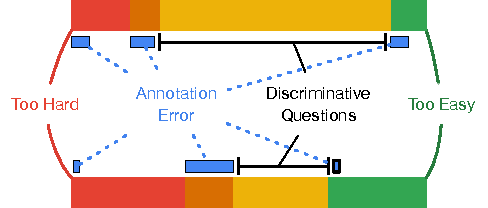
\includegraphics[width=1.0\linewidth]{figures/datasets/error_and_difficulty}
    \caption{Two datasets with $0.16$ annotation error: the top, however, better discriminates \abr{qa} ability.  In the good dataset (top), most questions are challenging but not impossible.  In the bad dataset (bottom), there are more trivial or impossible questions \emph{and} annotation error is concentrated on the challenging, discriminative questions.  Thus, a smaller fraction of questions decide who sits atop the leaderboard, requiring a larger test set.}
    \label{fig:error-and-difficulty}
\end{figure}

Figure~\ref{fig:error-and-difficulty} shows two datasets of the same size with the same annotation error.
However, they have different difficulty \emph{distributions} and \emph{correlation} of annotation error and difficulty.
The dataset that has more discriminative questions and consistent annotator error has fewer questions that do not discriminate the winner of the leaderboard.
We call this the effective dataset proportion~$\rho$ (higher is better).
Figure~\ref{fig:how-big} shows the test set size required to reliably discriminate systems for different $\rho$, based on a simulation (Appendix~\ref{sec:synthetic-discriminative}).

At this point, you may despair about how big a dataset you
need.\footnote{Using a more sophisticated simulation approach, the
  \abr{trec} 2002 \abr{qa} test set~\citep{voorhees-03} could not
  discriminate systems with less than a seven absolute score point
  difference.}
The same terror besets trivia tournament organizers.
Instead of writing more questions, they use pyramidality (Section~\ref{sec:pyramidality}) to make every question count.


\begin{figure*}[t!]
    \begin{center}
    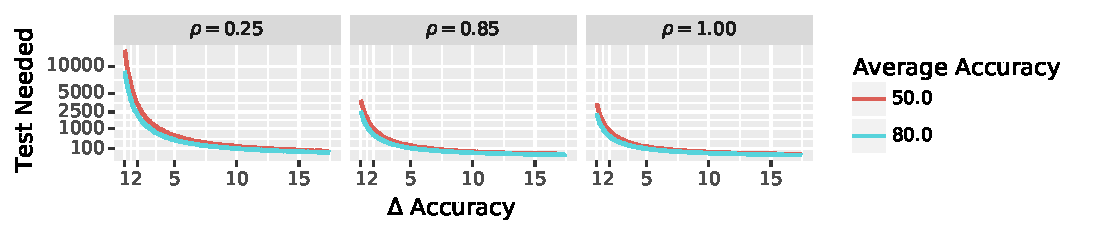
\includegraphics[width=1.0\linewidth]{figures/datasets/test_set}
    \end{center}
    \caption{
    How much test data do you need to discriminate two systems with 95\% confidence?  This depends on both the difference in accuracy between the systems ($x$ axis) and the average accuracy of the systems (closer to 50\% is harder).  Test set creators do not have much control over those.  They do have control, however, over how many questions are discriminative.  If all questions are discriminative (right), you only need 2500 questions, but if three quarters of your questions are too easy, too hard, or have annotation errors (left), you'll need 15000.}
    \label{fig:how-big}
\end{figure*}
\label{ch:adversarial}

\section{Adversarial Questions}
\label{sec:adversarial:adversarial}


\section{Human--Computer Cooperation}
\label{sec:adversarial:cooperation}


